\documentclass[12pt]{article}
\usepackage[a4paper, margin=1in]{geometry}
\usepackage{graphicx}
\usepackage{longtable}
\usepackage{titlesec}
\usepackage{caption}
\usepackage{booktabs}
\usepackage[colorlinks=true, linkcolor=blue, urlcolor=blue, citecolor=blue]{hyperref} % for clickable links

\title{\textbf{Technical Report - The Smart Boda Device}}
\author{
  Group 7 \\
  \\ 
  Watts Ryan Eric -- 24/U/20732/EVE -- 2400720732 \\
  Ssentaba Brian Kirabo -- 24/U/24769/PSA -- 2400724769 \\
  Akoragye Neville -- 24/U/03195/EVE -- 2400703195 \\
  Kazibwe David Nelson -- 24/U/24054/PS -- 2400724054 \\
  Mawanda John Paul -- 24/U/0678 -- 2400700678 \\
  \\ 
  Mentor: Mr. Paddy Asiimwe \\
  Course: CSC 1304 Practical Skills Development \\
  Date: July 13, 2025
}
\date{}

\begin{document}

\maketitle

\vspace{-1em} % tighten spacing after title

\tableofcontents

\vspace{1em} % space after ToC for neatness

\begin{abstract}
Uganda faces a high rate of road traffic accidents, with emergency response and reporting often delayed due to a lack of real-time detection and communication tools. The Smart Boda Device is a low-cost, sensor-based solution designed to detect likely accidents involving boda bodas in real time. By fusing data from accelerometers, gyroscopes, force sensors, and GPS, the device identifies crash events and transmits critical data to a Flutter-based web platform using Firebase and Firestore \cite{firebase}. This enables emergency responders and authorities to monitor incidents, analyze accident hotspots, and inform infrastructure improvements. The system is scalable and accessible, with potential for integration into fleet management and urban safety planning.
\end{abstract}

\newpage

\section{Introduction}
This report outlines the development and implementation of the Smart Boda Device, a real-time accident detection and alert system for boda bodas. The document details the user challenges, project goals, system requirements, and final outcomes. It also presents future work required to scale and improve the product.

\subsection{User Challenge}
Uganda's urban transport sector, particularly the boda boda industry, suffers from frequent accidents and delayed emergency responses. Current interventions lack real-time, automated detection and reporting, making it difficult for emergency services to respond promptly and for authorities to gather actionable data for policy and infrastructure improvements.

\subsection{Project Goals}
\begin{itemize}
  \item Develop a real-time accident detection system using sensor fusion (impact force, orientation, velocity, and acceleration) \cite{mpu6050}.
  \item Build a web-based platform for monitoring and alerting emergency responders using Flutter \cite{flutter}.
  \item Gather and analyze accident data to support future infrastructure and safety planning.
  \item Prototype a scalable, low-cost, and accessible hardware-software solution for widespread adoption.
\end{itemize}

\subsection{Functional Requirements}
\begin{itemize}
  \item \textbf{Accident Detection:} Identify crashes using data from accelerometer, gyroscope, force sensor, and GPS \cite{mpu6050}.
  \item \textbf{Data Transmission:} Send incident data to a web application in real time using GSM and cloud services.
  \item \textbf{Web Platform:} Visualize accident locations, historical data, and analytics for authorized users.
  \item \textbf{Data Storage:} Securely store all incident records using Firebase and Firestore \cite{firebase}.
  \item \textbf{Usability:} Ensure easy installation, low power consumption, and minimal rider interaction.
\end{itemize}

\section{Project Results}

\subsection{Product Design}
\textbf{Hardware Components:}
\begin{itemize}
  \item MPU6050 Sensor: 3-axis accelerometer and gyroscope for motion and orientation sensing \cite{mpu6050}.
  \item NEO-6MV2 GPS Module: Provides real-time location and velocity data.
  \item Force Sensor (FSR402/Piezoelectric): Detects impact magnitude, reducing false positives.
  \item ESP32 Microcontroller: Manages sensor data acquisition and processing.
  \item SIM800L GSM Module: Enables data transmission via cellular network.
  \item LiPo Battery: Rechargeable power source with voltage regulation.
\end{itemize}

\textbf{Software Components:}
\begin{itemize}
  \item Firmware: Implements sensor fusion, thresholding, and communication protocols.
  \item Web Application: Developed in Flutter, displays real-time alerts, mapping, and analytics \cite{flutter}.
  \item Backend: Firebase and Firestore for secure, scalable data storage and management \cite{firebase}.
\end{itemize}

\textbf{System Architecture:} 
Sensors collect data $\rightarrow$ ESP32 processes and evaluates thresholds $\rightarrow$ If an accident is detected, data is sent via GSM to Firebase $\rightarrow$ Web app visualizes and stores incidents.

\subsection{Product Functionality}
\begin{itemize}
  \item \textbf{Real-Time Alerts:} Immediate notification of detected accidents on the web platform.
  \item \textbf{Incident Mapping:} Visualization of accident locations for rapid response and analysis.
  \item \textbf{Historical Data Access:} Review and export past incident data for trend analysis.
  \item \textbf{User Management:} Access control for emergency responders, authorities, and analysts.
\end{itemize}

\subsubsection{Our basis for accident detection}
Our accident detection is based upon the following sensor readings and logic:

\begin{itemize}
  \item \textbf{Impact-force Readings:}  
  Readings above 3g (29.43 m/s\textsuperscript{2}) detected by the force sensor indicate a significant impact, likely caused by a collision rather than normal riding conditions. Such impacts include head-on collisions or collisions with stationary or moving objects.
  \begin{itemize}
    \item \textbf{Gyroscope Readings:}  
    A sudden sharp spike in angular velocity combined with accelerometer data suggests abnormal rotational movement typically experienced during a crash. This helps differentiate accidents from other movements.
    \item \textbf{Accelerometer Readings:}  
    High acceleration combined with force sensor triggers and gyro spikes confirms an accident event. Isolated acceleration spikes (e.g., over bumps) without corresponding gyro data are filtered out.
    \item \textbf{Sensor Fusion Logic:}  
    To reduce false positives, the system considers:  
    \begin{itemize}
      \item \textit{Speed bumps:} Cause acceleration spikes but no significant gyro spikes or force sensor impact.  
      \item \textit{Sharp turns:} Cause gyro spikes without large force impact or acceleration spikes indicating collisions.  
      \item \textit{Accident detection:} Requires concurrent detection of significant impact force, abnormal angular velocity (gyro spike), and sudden acceleration changes.  
    \end{itemize}
  \end{itemize}
\end{itemize}

\section{Limitations and Next Steps}

\subsection{Limitations}
\begin{itemize}
  \item Device operation depends on reliable cellular network coverage for real-time data transmission.
  \item False positives may occur due to extreme terrain vibrations, though mitigated by force sensor thresholding.
  \item Pilot deployment is limited in scale; broader testing is needed for full validation.
\end{itemize}

\subsection{Next Steps}
\begin{itemize}
  \item Refine detection algorithms and calibrate sensor thresholds using real-world feedback.
  \item Explore integration of alternative communication protocols for improved coverage.
  \item Expand deployment to a larger fleet and gather stakeholder input for further development.
  \item Investigate AI-based analytics and predictive modeling for proactive safety interventions.
\end{itemize}

\section*{References}
\begin{thebibliography}{9}

\bibitem{ieee} IEEE citation guide, \url{https://ieee.org/documents/ieeecitationref.pdf}

\bibitem{thingspeak} ThingSpeak IoT Analytics, \url{https://thingspeak.com}

\bibitem{mpu6050} MPU6050 Datasheet and Application Notes

\bibitem{flutter} Flutter Framework Documentation, \url{https://flutter.dev}

\bibitem{firebase} Firebase Documentation, \url{https://firebase.google.com}

\end{thebibliography}

\section*{Appendix A: Project Work Plan}

\begin{figure}[h!]
  \centering
  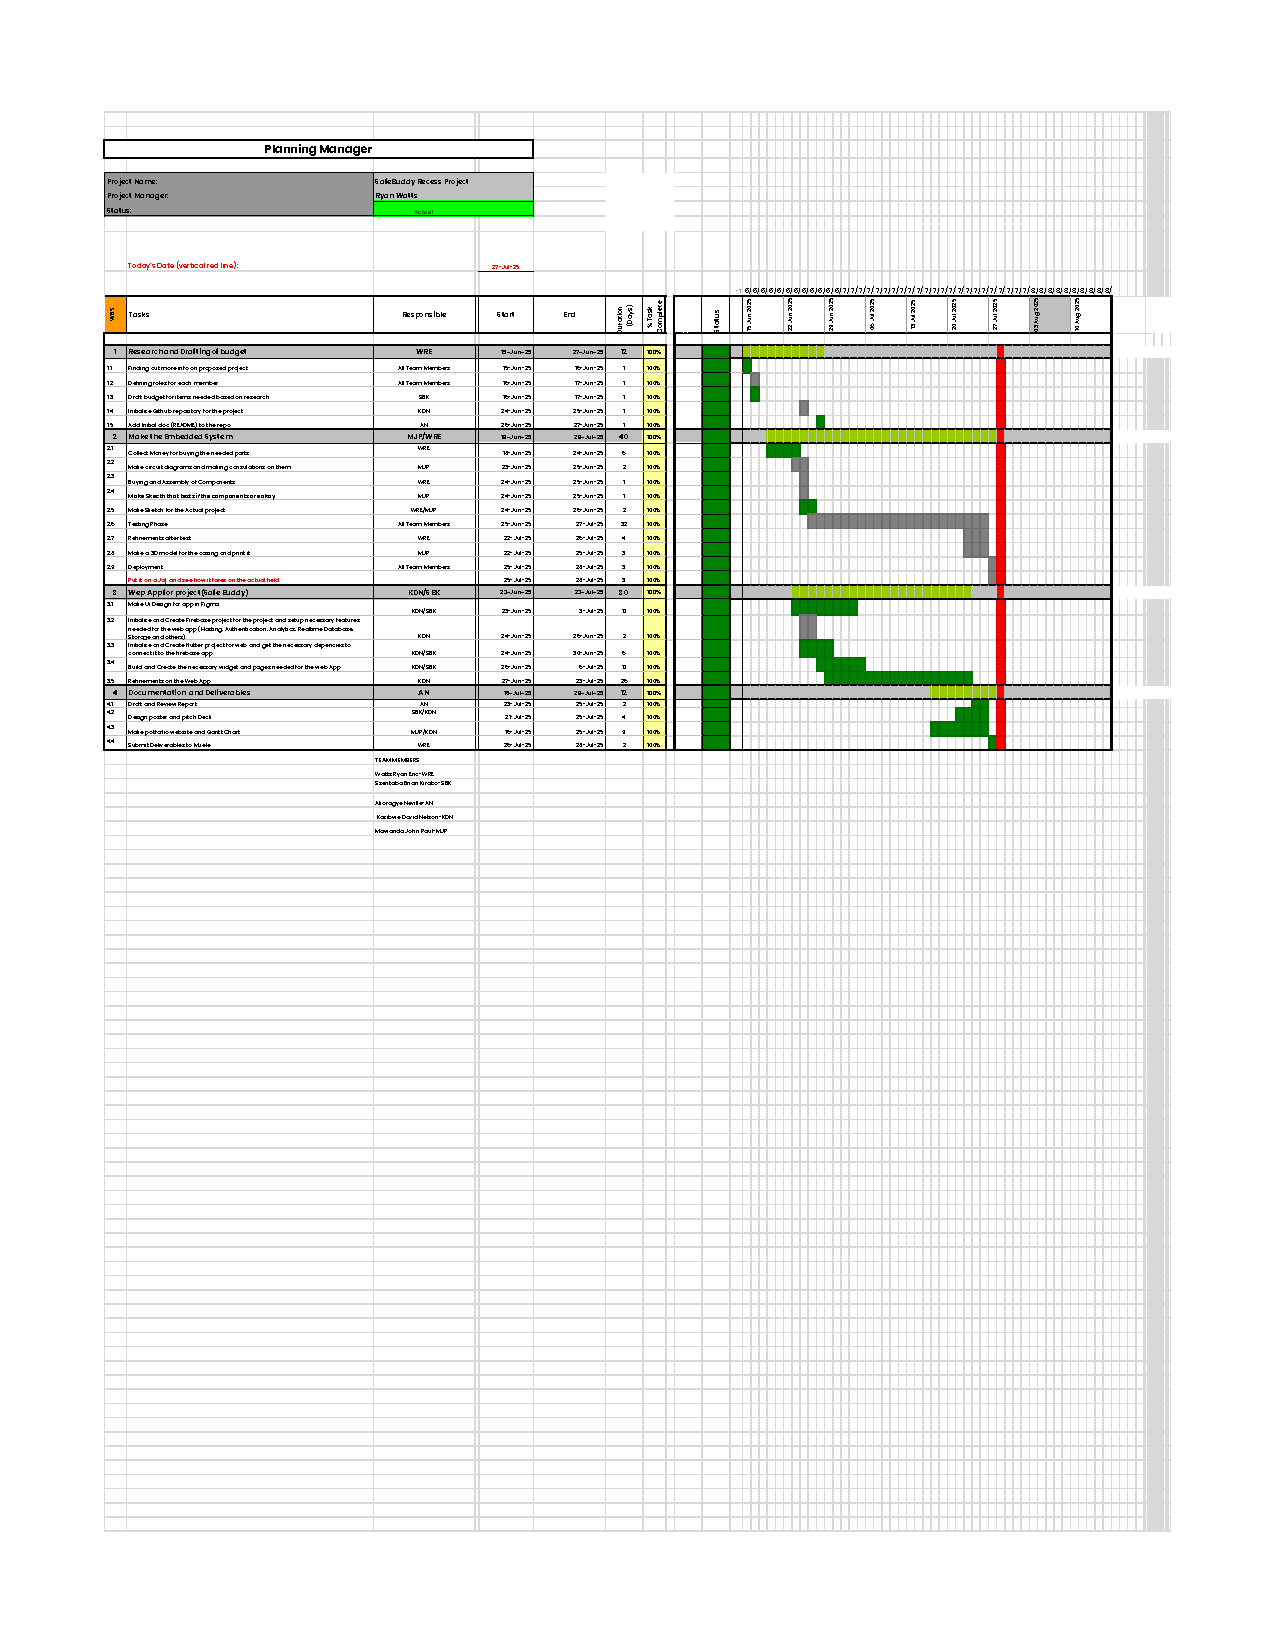
\includegraphics[width=\textwidth]{Gantt_Chart.pdf}
  \caption{Gantt Chart showing the SafeBuddy Recess Project Timeline}
  \label{fig:gantt}
\end{figure}

\section*{Appendix B: Contribution by Team Members}
\begin{longtable}{@{}ll@{}}
\toprule
\textbf{Team Member} & \textbf{Contribution} \\
\midrule
Watts Ryan Eric & Hardware \& Sensor integration \\
Ssentaba Brian Kirabo & GSM/GPS Communication and Backend setup \\
Akoragye Neville & Documentation and Testing \\
Kazibwe David Nelson & Web Platform and Flutter UI \\
Mawanda John Paul & Database integration \& Firebase \\
\bottomrule
\end{longtable}

\end{document}

